% ------------------------------------------------------------------
\documentclass[12 pt]{article} % A4 paper set by geometry package below
\pagenumbering{arabic}
\setlength{\parindent}{10 mm}
\setlength{\parskip}{12 pt}

% Nimbus Sans font should be reasonably legible
\usepackage{helvet}
\renewcommand{\familydefault}{\sfdefault}
\usepackage[T1]{fontenc}  % Without this \textsterling produces $

% Section header spacing
\usepackage{titlesec}
\titlespacing\section{0pt}{12pt plus 4pt minus 2pt}{0pt plus 2pt minus 2pt}
\titlespacing\subsection{0pt}{12pt plus 4pt minus 2pt}{0pt plus 2pt minus 2pt}
\titlespacing\subsubsection{0pt}{12pt plus 4pt minus 2pt}{0pt plus 2pt minus 2pt}

\usepackage{amsmath}
\usepackage{amssymb}
\usepackage{graphicx}
\usepackage{verbatim}    % For comment
\usepackage[paper=a4paper, marginparwidth=0 cm, marginparsep=0 cm, top=2.5 cm, bottom=2.5 cm, left=3 cm, right=3 cm, includemp]{geometry}
\usepackage[pdftex, pdfstartview={FitH}, pdfnewwindow=true, colorlinks=true, citecolor=blue, filecolor=blue, linkcolor=blue, urlcolor=blue, pdfpagemode=UseNone]{hyperref}

% Put module code and last-modified date in footer
\usepackage{fancyhdr}
\pagestyle{fancy}
\fancyhf{}
\renewcommand{\headrulewidth}{0pt}
\cfoot{{\small \thisunit}\hfill \thepage\hfill {\small \moddate}}

% Hopefully address Canvas complaints about pdf tagging
%\usepackage[tagged]{accessibility}
\hypersetup {
  pdfauthor={David Schaich},
  pdftitle={Statistical Physics Tutorial Activity},
}
% ------------------------------------------------------------------



% ------------------------------------------------------------------
% Shortcuts
\newcommand{\be}{\ensuremath{\beta} }
\newcommand{\eps}{\ensuremath{\varepsilon} }
\newcommand{\om}{\ensuremath{\omega} }
\newcommand{\pderiv}[2]{\ensuremath{\frac{\partial #1}{\partial #2}} }
% ------------------------------------------------------------------



% ------------------------------------------------------------------
\begin{document}
\newcommand{\thisunit}{MATH327 Tutorial (Lattice)}
\newcommand{\moddate}{Last modified 2 May 2024}
\begin{center}
  {\Large \textbf{MATH327: Statistical Physics, Spring 2024}} \\[12 pt]
  {\Large \textbf{Tutorial activity \ --- \ Lattices}} \\[24 pt]
\end{center}

This activity will be introduced in our 2 May tutorial, and you'll have until our final tutorial on 9 May to work on it.
You can already start considering the conceptual questions below, and in the next lecture we'll meet the Ising model on simple cubic lattices with periodic boundary conditions.
Other lattice structures play important roles in both nature and mathematics.
Some of the remarkable electronic properties of graphene, for example, are due to its two-dimensional honeycomb lattice structure, while more elaborate three-dimensional lattices play central roles in the search for materials exhibiting high-temperature superconductivity.

The figures below show three simple two-dimensional lattices, each of which has a different \textbf{coordination number} $C$ --- the number of nearest neighbours for each site (with periodic boundary conditions). % TODO: Adapted from doi.org/10.1007/978-3-319-10924-4_6
The square lattice has $C = 2d = 4$, and generalizes to simple cubic and hyper-cubic lattices in higher dimensions.

\begin{center}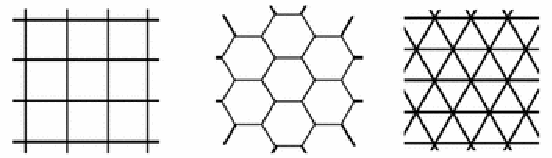
\includegraphics[width=\textwidth]{figs/lattices.pdf}\end{center}

The honeycomb lattice of graphene has a smaller $C = d + 1 = 3$, and generalizes to `hyper-diamond' lattices in higher dimensions.
Finally, the triangular lattice essentially fills in the middle of each honeycomb cell, leading to coordination number $C = 2(d + 1) = 6$.
Its higher-dimensional generalizations are known as $A_d^*$ lattices, of which the simplest example is the three-dimensional body-centered cubic lattice shown below.
Also shown below is the 2d `kagome' lattice, which has the same $C = 4$ as the square lattice, illustrating that the coordination number is insufficient to completely characterize a lattice.

\begin{center}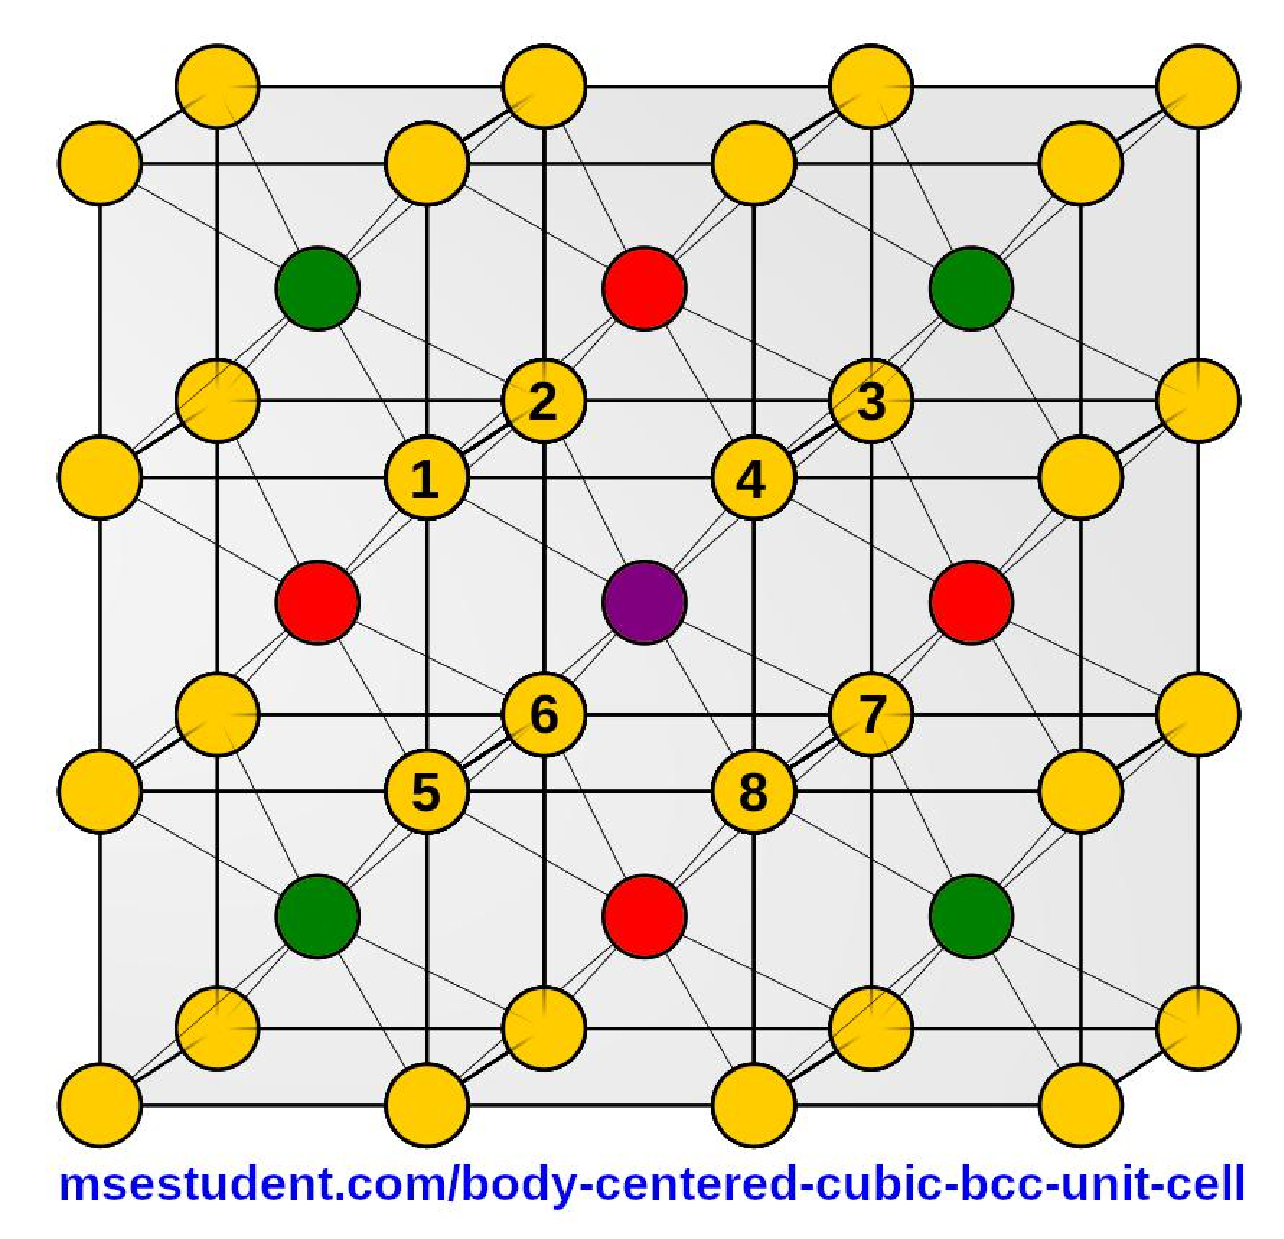
\includegraphics[width=0.35\textwidth]{figs/bcc.pdf}\hspace{0.25\textwidth}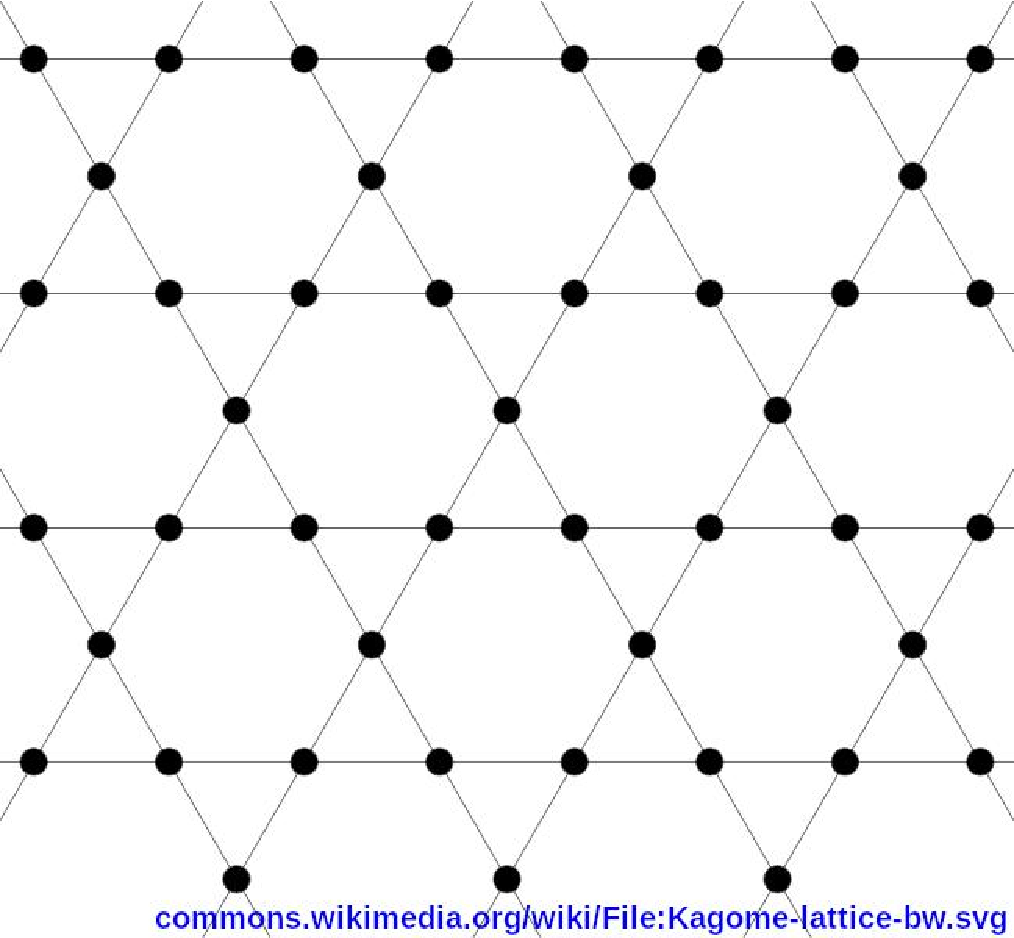
\includegraphics[width=0.35\textwidth]{figs/kagome.pdf}\end{center}

We can define versions of the Ising model with nearest neighbours $(jk)$ given by any of the lattices shown above.
We can further generalize the Ising model to have energy
\begin{equation*}
  E = -J \sum_{(jk)} s_j s_k - H \sum_{n = 1}^N s_n,
\end{equation*}
where $J$ sets the interaction strength.
While any positive $J > 0$ can be rescaled to our usual $J = 1$ without loss of generality, the case of a constant negative $J < 0$ is qualitatively different.
Setting $H = 0$, consider the following \textbf{conceptual questions} without doing detailed calculations:
What are the minimum-energy ground states for each case $J > 0$ and $J < 0$, for each of the square, honeycomb and triangular lattices?
What sort of order parameter could distinguish these ground states from the disordered micro-states that dominate at high temperatures?

Generalizing the Ising model in this way opens up a vast landscape of applications.
One important example is modelling \textbf{spin glasses}, by allowing the interaction strength to vary from link to link:
\begin{equation*}
  E_{\text{SG}} = -\sum_{(jk)} J_{jk} s_j s_k.
\end{equation*}
Giorgio Parisi was awarded part of the 2021 Nobel Prize in Physics for his work studying the mathematics of such spin glass systems.
In particular, he was able to solve the system for which (1) the values $J_{jk}$ are randomly drawn from a gaussian distribution around some mean $J_0$, and (2) every site $j$ is a nearest neighbour of every other site $k \ne j$, giving a fully connected lattice (or \textbf{complete graph}).
The pictures on the next page illustrate complete graphs with $N = 1, 2, \cdots, 12$ sites, for which the sum over links turns into a sum over all $1 \leq j < k \leq N$.
How many links are there for $N$ sites in this case?

Spin glasses are too complicated to tackle here.
Instead, let's return to a simpler Ising model with constant interaction strength, while still considering the fully connected lattice:
\begin{equation*}
  E = -\frac{J}{N} \sum_{j < k} s_j s_k - H \sum_{n = 1}^N s_n = -\frac{J}{2N} \sum_{j \neq k} s_j s_k - H \sum_{n = 1}^N s_n.
\end{equation*}
We normalize the interaction strength by $N$ so that the system retains a finite energy per spin in the $N \to \infty$ thermodynamic limit.

\textbf{The challenge} is to solve this Ising model on the fully connected lattice --- that is, to compute a closed-form expression for its partition function $Z$.
This is tricky, but can be done by writing $Z$ as a sum over the $N + 1$ possible values of the magnetization $-1 \leq m \leq 1$, and counting how many micro-states there are for each magnetization.
The energy above also needs to expressed in terms of the magnetization, which is easier to do by considering the sum over all $j \neq k$.
Finally, for large $N$ we can approximate the $N + 1$ possible values of $m$ as continuously varying, and integrate
\begin{equation*}
  Z = \int_{-1}^1 \ (\cdots) \ dm.
\end{equation*}

\begin{center}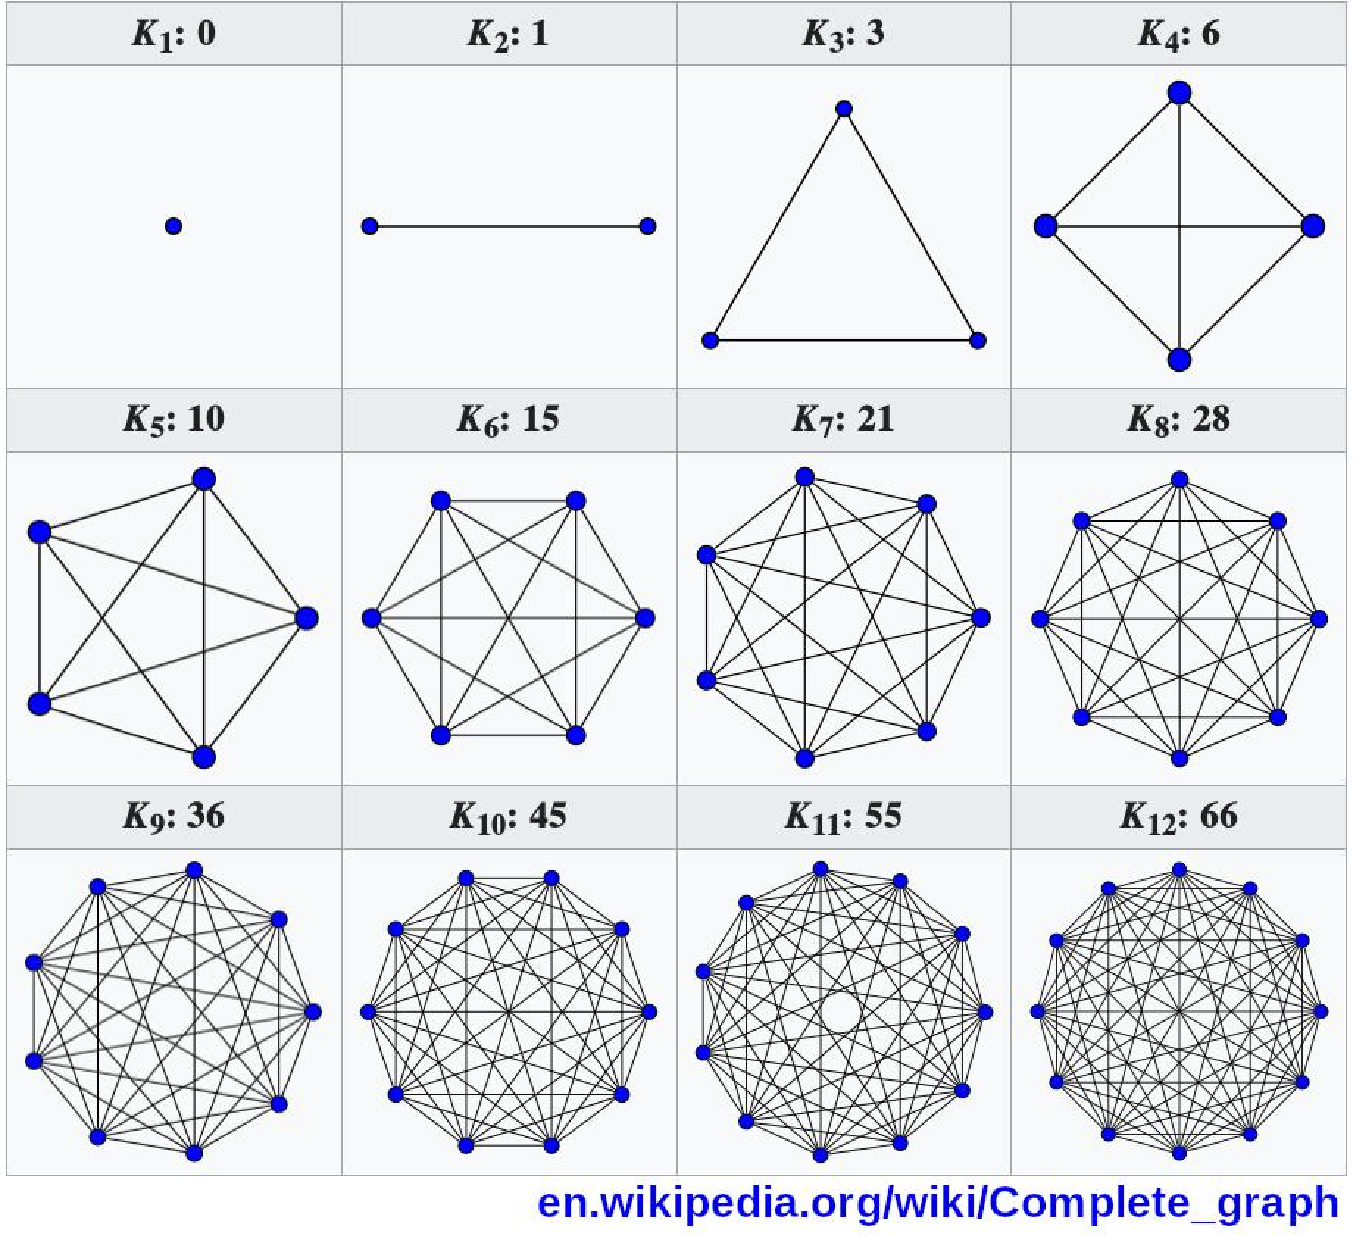
\includegraphics[width=\textwidth]{figs/completeGraph.pdf}\end{center}

\end{document}
% ------------------------------------------------------------------
